En este TP se lleva a cabo el análisis de distintas redes a partir de
la captura de paquetes, modelándolos de diversas formas utilizando
conceptos de la teoría de la información.
 
Un concepto importante en este contexto es el de \textit{información}. Sea $E$
un evento que ocurre con probabilidad $P(E)$. Decimos que al ocurrir
dicho evento hemos recibido

$$
I(E) = \log{\frac{1}{P(E)}}
$$
unidades de información.
 
Según la base del logaritmo usada sea $10$, $e$, o $2$, decimos que
hemos recibido Hartleys, nats, o bits.
 
Otro concepto importante es el de fuente de información con 
\textit{memoria nula}.
Una fuente de este tipo emite una secuencia de símbolos
provenientes de un alfabeto fijo de un tamaño finito $S
= \{s_1, \dots, s_n\}$, cada uno de los cuales tiene una probabilidad
de ocurrencia fija. Se dice que tiene "memoria nula" porque la
probabilidad de emitir un símbolo cualquiera es independiente de los
símbolos emitidos anteriormente.

Un concepto ligado una una fuente así definida es el de \textit{entropía}, que
es la suma de la información asociada a cada símbolo multiplicada por
su probabilidad; es decir:
$$
H(S) = \sum_{s \in S} P(s)I(s)
$$

Por último, una propiedad que vamos a tener en cuenta en nuestro
trabajo es que el valor máximo de la entropía (dada una fuente y
variando las probabilidades) es $log |S|$; valor que
alcanza cuando todos los símbolos son equiprobables.

\subsection{Frames Ethernet y el protocolo ARP}

Los paquetes de red (Ethernet) que capturamos, se componen principalmente de un campo conocido como EtherType

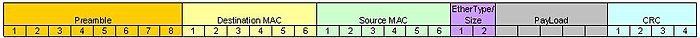
\includegraphics[scale=0.6]{Ether.jpg}

Esto no ayuda saber que tipo de protocolo esta encapsulado dentro del paquete. Por lo general dentro de los paquetes pueden existen distintos tipos protocolos. Lo que mas se quiere caracterizar en este, es aquellos que usan el protocolo ARP.

\subsubsection(ARP)


El protocolo ARP trabaja entre la capa de enlace y la capa red. Es el encargado de mapear las direcciones IP de la red, de modo que esten asociadas con las direcciones MAC de la red.
Los paquetes que usa el protocolo ARP pueden ser de tipo broadcast o de tipo unicast. Las tipo Broadcast o Who-has es un request con destino ff:ff:ff:ff:ff:ff que pregunta que direccion ip tiene cierta direccion MAC. Las de tipo unicast son reply que responden con la direccion MAC a quien pregunto por cierta direccion IP.

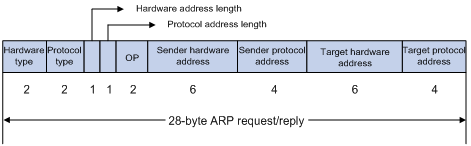
\includegraphics[scale=0.8]{arp.png}

Toda este intercambio de paquetes ayuda a armar la tabla de direcciones MAC e IP que forman una red.
   
